\documentclass[11pt,a4paper]{report}
\usepackage{hyperref}
\usepackage[margin=2.5cm]{geometry}
\usepackage{amsmath, amsthm}
\usepackage{txfonts}
\usepackage{todonotes}
\usepackage{enumitem}
\usepackage{listings}
\usepackage[nameinlink]{cleveref}
\usepackage{microtype}
\usepackage[group-separator={,}]{siunitx}

\hypersetup{
  pdftitle={The Bcc Consensus and Storage Layer},
  pdfborder={0 0 0},
  breaklinks=true
}

\usetikzlibrary{arrows.meta}
\usetikzlibrary{intersections}

% https://tex.stackexchange.com/questions/229940/can-i-have-a-listing-with-fixed-column-code-and-full-flexible-comments
\makeatletter
\let\commentfullflexible\lst@column@fullflexible
\makeatother

% Use continuous footnote numbering so we can refer to them
% https://tex.stackexchange.com/questions/10448/continuous-footnote-numbering
\counterwithout{footnote}{chapter}

\lstset{
    language=haskell
  , basicstyle=\small\ttfamily
  , keywordstyle=\bfseries
  , commentstyle=\normalsize\rmfamily\itshape\commentfullflexible
  , columns=fixed
  , morekeywords={
        family
      , Type
      }
  }

\theoremstyle{definition}
\newtheorem{property}{Property}
\newtheorem{definition}{Definition}
\newtheorem{lemma}{Lemma}
\newtheorem{assumption}{Assumption}
\newtheorem{corollary}{Corollary}
\newtheorem{proposal}{Proposal}
\newtheorem{failedattempt}{Failed attempt}
\numberwithin{property}{chapter}
\numberwithin{definition}{chapter}
\numberwithin{lemma}{chapter}
\numberwithin{assumption}{chapter}
\numberwithin{corollary}{chapter}
\numberwithin{proposal}{chapter}
\numberwithin{failedattempt}{chapter}

\newenvironment{bug}
  {\begin{quote} \textbf{Known bug}.}
  {\end{quote}}

\title{The Bcc Consensus and Storage Layer \\
       {\large \sc An TBCO technical report}
  }
\author{Edsko de Vries \\ \href{mailto:edsko@well-typed.com}
                               {\small \texttt edsko@well-typed.com}
   \and Thomas Winant  \\ \href{mailto:thomas@well-typed.com}
                               {\small \texttt thomas@well-typed.com}
   \and rmourey_jr Coutts  \\ \href{mailto:duncan@well-typed.com}
                               {\small \texttt duncan@well-typed.com}
                       \\ \href{mailto:duncan.coutts@blockchain-company.io}
                               {\small \texttt duncan.coutts@blockchain-company.io}
  }

\newcommand{\debugsep}[1]{
  \vspace{2em}
  \hrule
  \vspace{0.5em}
  \textbf{#1}
  \vspace{0.5em}
  \hrule
  \vspace{2em}
}

% TODO
%
% * Incorporate
%
%   - Previous blog posts
%   - Specifications currently stored as markdown files in the repo
%   - Any discussions in long comments in the code
%
% - choice of k: liveness versus safety
% - make sure we talk about the fact that the ledger can be linear

\newcommand{\duncan}{\todo{rmourey_jr suitable section.}}

\begin{document}

\maketitle

\tableofcontents

\input{chapters/intro/intro.tex}
\chapter{Overview}

\section{Components}

\subsection{Consensus protocols}
\label{overview:consensus}

The consensus protocol has two primary responsibilities:
\label{consensus-responsibilities}

\begin{description}
\item[Chain selection] Competing chains arise when two or more nodes extend the
chain with different blocks. This can happen when nodes are not aware of each
other's blocks due to temporarily network delays or partitioning, but depending
on the particular choice of consensus algorithm it can also happen in the normal
course of events. When it happens, it is the responsibility of the consensus
protocol to choose between these competing chains.

\item[Leadership check] In proof-of-work blockchains any node can produce a
block at any time, provided that they have sufficient hashing power. By
contrast, in proof-of-stake time is divided into \emph{slots}, and each slot has
a number of designated \emph{slot leaders} who can produce blocks in that slot.
It is the responsibility of the consensus protocol to decide on this mapping
from slots to slot leaders.
\end{description}

The consensus protocol will also need to maintain its own state; we will discuss
state management in more detail in \cref{storage:inmemory}.

\subsection{Ledger}
\label{overview:ledger}

The role of the ledger is to define what is stored \emph{on} the blockchain.
From the perspective of the consensus layer, the ledger has three primary
responsibilities:

\begin{description}
\item[Applying blocks] The most obvious and most important responsibility of
the ledger is to define how the ledger state changes in response to new blocks,
validating blocks at it goes and rejecting invalid blocks.\

\item[Applying transactions] Similar to applying blocks, the ledger layer also
must provide an interface for applying a single transaction to the ledger state.
This is important, because the consensus layer does not just deal with
previously constructed blocks, but also constructs \emph{new} blocks.

\item[Ticking time] Some parts of the ledger state change due to the passage of
time only. For example, blocks might \emph{schedule} some changes to be applied
later, and then when the relevant slot arrives those changes should be applied,
independent from any blocks.

\item[Forecasting] Some consensus protocols require limited information from the
ledger. In Optimum, for example, a node's probability of being a slot leader is
proportional to its stake, but the stake distribution is something that the
ledger keeps track of. We refer to this as a \emph{view} on the ledger, and we
require not just that the ledger can give us a view on the \emph{current} ledger
state, but also \emph{predict} what that view will be for slots in the near
future. We will discuss the motivation for this requirement in
\cref{nonfunctional:network:headerbody}.
\end{description}

The primary reason for separating out ``ticking'' from applying blocks is that
the consensus layer is responsible to the leadership check
(\cref{consensus-responsibilities}), and when we need to decide if we should be
producing a block in a particular slot, we need to know the ledger state at that
slot (even though we don't have a block for that slot \emph{yet}). It is also
required in the mempool; see \cref{mempool}.

\section{Design Goals}

\subsection{Multiple consensus protocols}
\label{multiple-consensus-protocols}

From the beginning it was clear that we would need support for multiple
consensus algorithms: the Cole era uses a consensus algorithm called
(Permissive) BFT (\cref{bft}) and the Sophie era uses a consensus algorithm
called Optimum (\cref{optimum}). Moreover, the Bcc blockchain is a \emph{hybrid}
chain where the prefix of the chain runs Cole (and thus uses BFT), and then
continues with Sophie (and thus uses Optimum); we will come back to the topic of
composing protocols when we discuss the hard fork combinator (\cref{hfc}). It is
therefore important that the consensus layer abstracts over a choice of
consensus protocol.

\subsection{Support for multiple ledgers}
\label{multiple-ledgers}

For much the same reason that we must support multiple consensus protocols, we
also have to support multiple ledgers. Indeed, we expect more changes in ledger
than in consensus protocol; currently the Bcc blockchain starts with a
Cole ledger and then transitions to a Sophie ledger, but further changes to
the ledger have already been planned (some intermediate ledgers currently
code-named Evie and Jen, as well as larger updates to Charles, Brandon and
Sjobs). All of the ledgers (Sophie up to including Sjobs)
use the Optimum consensus algorithm (potentially extended with the genesis chain
selection rule, see \cref{genesis}).

\subsection{Decouple consensus protocol from ledger}
\label{decouple-consensus-ledger}

As we saw above (\cref{multiple-ledgers}), we have multiple ledgers that all
use the same consensus protocol. We therefore should be able to define the
consensus protocol \emph{independent} from a particular choice of ledger,
merely defining what the consensus protocol expects from the ledger
(we will see what this interface looks like in \cref{ledger}).

\subsection{Testability}
\label{testability}

The consensus layer is a critical component of the Bcc Node, the software
that runs the Bcc blockchain. Since the blockchain is used to run the bcc
cryptocurrency, it is of the utmost importance that this node is reliable;
network downtime or, worse, corruption of the blockchain, cannot be tolerated.
As such the consensus layer is subject to much stricter correctness criteria
than most software, and must be tested thoroughly. To make this possible, we
have to design for testability.

\begin{itemize}
\item We must be able to simulate various kinds of failures (disk
failures, network failures, etc.) and verify that the system can recover.
\item We must be able to run \emph{lots} of tests which means that tests need to
be cheap. This in turn will require for example the possibility to swap the
cryptographic algorithms for much faster ``mock'' crypto algorithms.
\item We must be able to test how the system behaves under certain
expected-but-rare circumstances. For example, under the Optimum consensus
protocol it can happen that a particular slot has multiple leaders. We should be
able to test what happens when this happens repeatedly, but the leader selection
is a probabilistic process; it would be difficult to set up test scenarios to
test for this specifically, and even more difficult to set things up so that
those scenarios are \emph{shrinkable} (leading to minimal test cases). We must
therefore be able to ``override'' the behaviour of the consensus protocol (or
indeed the ledger) at specific points.
\item We must be able to test components individually (rather than just the
system as a whole), so that if a test fails, it is much easier to see where
something went wrong.
\end{itemize}

\subsection{Adaptability and Maintainability}
\label{adaptability}

The Bcc Node began its life as an ambitious replacement of the initial
implementation of the Bcc blockchain, which had been developed by Serokell.
At the time, the Sophie ledger was no more than a on-paper design, and
the Optimum consensus protocol existed only as a research paper. Moreover, since
the redesign would be unable to reuse any parts of the initial implementation,
even the Cole ledger did not yet exist when the consensus layer was started.
It was therefore important from the get-go that the consensus layer was not
written for a specific ledger, but rather abstract over a choice of ledger
and define precisely what the responsibilities of that ledger were.

This abstraction over both the consensus algorithm and the ledger is important
for other reasons, too. As we've mentioned, although initially developed to
support the Cole ledger and the (Permissive) BFT consensus algorithm, the goal
was to move to Sophie/Optimum as quickly as possible. Moreover, additional
ledgers had already been planned (Charles, Brandon and Sjobs), and research on
consensus protocols was (and still is) ongoing. It was therefore important that
the consensus layer could easily be adapted.

Admittedly, adaptability does not \emph{necessarily} require abstraction. We
could have built the consensus layer against the Cole ledger initially
(although we might have had to wait for it to be partially completed at least),
and then generalise as we went. There are however a number of downsides to this
approach.

\begin{itemize}
\item When working with a concrete interface, it is difficult to avoid certain
assumptions creeping in that may hold for this ledger but will not hold for
other ledgers necessarily. When such assumptions go unnoticed, it can be costly
to adjust later. (For one example of such an assumption that nonetheless
\emph{did} go unnoticed, despite best efforts, and took a lot of work to
resolve, see \cref{time} on removing the assumption that we can always
convert between wallclock time and slot number.)

\item TBCO is involved in the development of blockchains other than the public
Bcc instance, and from the start of the project, the hope was that the
consensus layer can be used in those projects as well. Indeed, it is currently
being integrated into various other TBCO projects.

\item Perhaps most importantly, if the consensus layer only supports a single,
concrete ledger, it would be impossible to \emph{test} the consensus layer with
any ledgers other than that concrete ledger. But this means that all consensus
tests need to deal with all the complexities of the real ledger. By contrast,
by staying abstract, we can run a lot of consensus tests with mock ledgers that
are easier to set up, easier to reason about, more easily instrumented and more
amenable to artificially creating rare circumstances (see \cref{testability}).
\end{itemize}

Of course, abstraction is also just good engineering practice. Programming
against an abstract interface means we are clear about our assumptions,
decreases dependence between components, and makes it easier to understand and
work with individual components without having to necessarily understand the
entire system as a whole.

\subsection{Composability}
\label{composability}

The consensus layer is a complex piece of software;  at the time we are writing
this technical report, it consists of roughly 100,000 lines of code. It is
therefore important that we split it into into small components that can be
understood and modified independently from the rest of the system. Abstraction,
discussed in \cref{adaptability}, is one technique to do that, but by no means
the only. One other technique that we make heavy use of is composability. We
will list two examples here:

\begin{itemize}
\item As discussed in \cref{multiple-consensus-protocols} and
\cref{multiple-ledgers}, the Bcc blockchain has a prefix that runs the BFT
consensus protocol and the Cole ledger, and then continues with the Optimum
consensus protocol and the Sophie ledger. We do not however define a consensus
protocol that is the combination of Cole and Optimum, nor a ledger that is the
combination of Cole and Sophie. Instead, the \emph{hard fork combinator}
(\cref{hfc}) makes it possible to \emph{compose} consensus protocols and
ledgers: construct the hybrid consensus protocol from an implementation of BFT
and an implementation of Optimum, and similarly for the ledger.

\item We mentioned in \cref{testability} that it is important that we can
test the behaviour of the consensus layer under rare-but-possible circumstances,
and that it is therefore important that we can override the behaviour of the
consensus algorithm in tests. We do not accomplish this however by adding
special hooks to the Optimum consensus algorithm (or any other); instead we define
another combinator that takes the implementation of a consensus algorithm and
\emph{adds} additional hooks for the sake of the testing infrastructure. This
means that the implementation of Optimum does not have to be aware of testing
constraints, and the combinator that adds these testing hooks does not need to
be aware of the details of how Optimum is implemented.
\end{itemize}

\subsection{Predictable Performance}

Make sure node operators do not set up nodes for "normal circumstances" only
for the network to go down when something infrequent (but expected) occurs.
(This is not about malicious behaviour, that's the next section).

\duncan

\subsection{Protection against DoS attacks}

Brief introduction to asymptotic attacker/defender costs. (This is just an
overview, we come back to these topics in more detail later.)

\duncan

\section{History}
\label{overview:history} % OBFT references refer to this section as well

\duncan

\begin{itemize}
\item Briefly describe the old system (\lstinline!bcc-sl!) the decision
to rewrite it
\item Briefly discuss the OBFT hard fork.
\end{itemize}

\chapter{Non-functional requirements}
\label{nonfunctional}

This whole chapter is rmourey_jr-suitable :)
\duncan

\section{Network layer}
\label{nonfunctional:network}

This report is not intended as a comprehensive discussion of the network layer;
see \cite{network-spec} instead. However, in order to understand
some of the design decisions in the consensus layer we need to understand some
of the requirements imposed on it by the network layer.

TODOs:

\begin{itemize}
\item Highlight relevant aspects of the design of the network layer
\item Discuss requirements this imposes on the consensus layer
Primary example: Forecasting.
\item How do we keep the overlap between network and consensus as small
as possible? Network protocols do not involve consensus protocols
(chain sync client is not dependent on chain selection). Chain sync
client + "pre chain selection" + block download logic keeps things isolated.
\item Why do we even want to validate headers ahead of time? (Thread model etc.)
(Section for rmourey_jr?).
Section with a sketch on an analysis of the amortised cost for attackers versus
our own costs to defend against it ("budget for work" that grows and shrinks
as you interact with a node).
\end{itemize}

\subsection{Header/Body Split (aka: Header submission)}
\label{nonfunctional:network:headerbody}

Discuss the chain fragments that we store per upstream node.
Discuss why we want to validate headers here -- without a full ledger state
(necessarily so, since no block bodies -- can't update ledger state): to prevent
DoS attacks.
(\cref{ledger:forecasting} contains a discussion of this from the point of view of
the ledger).
Forward reference to the chain sync client (\cref{chainsyncclient}).
Discuss why it's useful if the chain sync client can race ahead  for
\emph{performance} (why it's required for chain selection is the discussed in
\cref{forecast:ledgerview}).

See also section on avoiding the stability window
(\cref{low-density:pre-genesis}).

\subsection{Block submission}
\label{nonfunctional:network:blocksubmission}

Forward reference to \cref{servers:blockfetch}.

\subsection{Transaction submission}
\label{nonfunctional:network:txsubmission}

Mention that these are defined entirely network side, no consensus involvement
(just an abstraction over the mempool).

\section{Security "cost" concerns}

TODO: Look through the code and git history to find instances of where we
one way but not the other because it would give an attacker an easy way to
make it do lots of work (where were many such instances).

Fragile. Future work: how might be make this less brittle?
Or indeed, how might we test this?

Counter-examples (things we don't want to do)

\begin{itemize}
\item Parallel validation of an entire epoch of data (say, crypto only).
You might do a lot of work before realising that that work was not needed because
of an invalid block in the middle.
\end{itemize}

Future work: opportunities for parallelism that we don't yet exploit
(important example: script evaluation in Charles).

\section{Hard time constraints}

Must produce a block on time, get it to the next slot leader

Bad counter-example: reward calculation in the Sophie ledger bad
(give examples of why).

\section{Predictable resource requirements}
\label{nonfunctional:best-is-worst}

make best == worst

(not \emph{just} a security concern: a concern even if every node honest)


\part{Consensus Layer}

\input{chapters/consensus/protocol.tex}
\chapter{Interface to the ledger}
\label{ledger}

\section{Abstract interface}
\label{ledger:api}

In \cref{overview:ledger} we identified three responsibilities for the ledger
layer:
%
\begin{itemize}
\item ``Ticking'' the ledger state, applying any time related changes
(\cref{ledger:api:IsLedger}). This is independent from blocks, both at the value
level (we don't need a block in order to tick) and at the type level.
\item Applying and verifying blocks (\cref{ledger:api:ApplyBlock}). This
obviously connects a ledger and a block type, but we try to avoid to talk about
\emph{the} ledger corresponding to a block, in order to improve
compositionality; we will see examples of where this comes in useful in the
definition of the extended ledger state (\cref{storage:extledgerstate}) and the
ledger database (\cref{ledgerdb}).
\item Projecting out the ledger view (\cref{ledger:api:LedgerSupportsProtocol}),
connecting a ledger to a consensus protocol.
\end{itemize}
%
We will discuss these responsibilities one by one.

\subsection{Independent definitions}
\label{ledger:api:IsLedger}

We will start with ledger API that can be defined independent of a choice of
block or a choice of consensus protocol.

\subsubsection{Configuration}

Like the other abstractions in the consensus layer, the ledger defines its own
type of required static configuration
%
\begin{lstlisting}
type family LedgerCfg l :: Type
\end{lstlisting}

\subsubsection{Tip}

We require that any ledger can report its tip as a \lstinline!Point!. A
\lstinline!Point! is either genesis (no blocks have been applied yet) or a pair
of a hash and slot number; it is parametric over $l$ in order to allow
different ledgers to use different hash types.
%
\begin{lstlisting}
class GetTip l where
  getTip :: l -> Point l
\end{lstlisting}

\subsubsection{Ticking}

We can now define the \lstinline!IsLedger! class as
%
\begin{lstlisting}
class (GetTip l, GetTip (Ticked l), ..) => IsLedger l where
  type family LedgerErr l :: Type
  applyChainTick :: LedgerCfg l -> SlotNo -> l -> Ticked l
\end{lstlisting}

The type of \lstinline!applyChainTick! is similar to the type of
\lstinline!tickChainDepState! we saw in \cref{consensus:class:state}.
Examples of the time-based changes in the ledger state include activating
delegation certificates in the Cole ledger, or paying out staking rewards
in the Sophie ledger.

Ticking is not allowed to fail (it cannot return an error). Consider what it
would mean if it \emph{could} fail: it would mean that a previous block was
accepted as valid, but set up the ledger state so that no matter what would
happen next, as soon as a particular moment in time is reached, the ledger would
fail to advance any further. Obviously, such a situation cannot be permitted to
arise (the block should have been rejected as invalid).

Note that ticking does not change the tip of the ledger: no blocks have been
applied (yet). This means that we should have

\begin{equation}
  \mathtt{getTip} \; l
= \mathtt{getTip} \; (\mathtt{applyChainTick}_\mathit{cfg} \; s \; l)
\end{equation}

\subsubsection{Ledger errors}

The inclusion of \lstinline!LedgerErr! in \lstinline!IsLedger! is perhaps
somewhat surprising. \lstinline!LedgerErr! is the type of errors that can arise
when applying blocks to the ledger, but block application is not yet defined
here. Nonetheless, a ledger can only be used with a \emph{single} type of
block\footnote{While it is true that the Bcc ledger can be used with Cole
blocks, Sophie blocks, Charles blocks, etc., this distinction between the
different blocks is invisible to most of the consensus layer. The whole raison
d'\^{e}tre of the hard fork combinator (\cref{hfc}) is to present a composite
ledger (say, the one consisting of the Cole, Sophie and Charles eras) as a
single type of ledger with a single type of block. The rest of the consensus
layer is not aware that this composition has happened; from its point
perspective it's just another ledger with an associated block type.}, and
consequently can only have a \emph{single} type of error; the only reason block
application is defined separately is that a single type of \emph{block} can be
used with multiple ledgers (in other words, this is a 1-to-many
relationship).\footnote{Defining \lstinline!LedgerErr! in \lstinline!ApplyBlock!
(\cref{ledger:api:ApplyBlock}) would result in ambiguous types, since it would
not refer to the \lstinline!blk! type variable of that class.}

\subsection{Applying blocks}
\label{ledger:api:ApplyBlock}

If \lstinline!applyChainTick! was analogous to \lstinline!tickChainDepState!,
then \lstinline!applyLedgerBlock! and \lstinline!reapplyLedgerBlock! are
analogous to \lstinline!updateChainDepState! and
\lstinline!reupdateChainDepState!, respectively
(\cref{consensus:class:state}): apply a block to an already ticked
ledger state:
%
\begin{lstlisting}
class (IsLedger l, ..) => ApplyBlock l blk where
  applyLedgerBlock ::
    LedgerCfg l -> blk -> Ticked l -> Except (LedgerErr l) l
  reapplyLedgerBlock ::
    LedgerCfg l -> blk -> Ticked l -> l
\end{lstlisting}
%
The discussion of the difference between, and motivation for, the distinction
between application and reapplication in \cref{consensus:class:state}
about the consensus protocol state applies here equally.

\subsection{Linking a block to its ledger}

We mentioned at the start of \cref{ledger:api} that a single block can be used
with multiple ledgers. Nonetheless, there is one ``canonical'' ledger for each
block; for example, the Sophie block is associated with the Sophie ledger,
even if it can also be applied to the extended ledger state or the ledger
DB. We express this through a data family linking a block to its ``canonical
ledger state'':
%
\begin{lstlisting}
data family LedgerState blk :: Type
\end{lstlisting}
%
and then require that it must be possible to apply a block to its associated
ledger state
%
\begin{lstlisting}
class ApplyBlock (LedgerState blk) blk => UpdateLedger blk
\end{lstlisting}
%
(this is an otherwise empty class). For convenience, we then also introduce
some shorthand:
%
\begin{lstlisting}
type LedgerConfig      blk = LedgerCfg (LedgerState blk)
type LedgerError       blk = LedgerErr (LedgerState blk)
type TickedLedgerState blk = Ticked    (LedgerState blk)
\end{lstlisting}

\subsection{Projecting out the ledger view}
\label{ledger:api:LedgerSupportsProtocol}

In \cref{overview:ledger} we mentioned that a consensus protocol may require
some information from the ledger, and in \cref{consensus:class:ledgerview} we
saw that this is modelled as the \lstinline!LedgerView! type family in the
\lstinline!ConsensusProtocol! class. A ledger and a consensus protocol are
linked through the block type (indeed, apart from the fundamental concepts we
have discussed so far, most of consensus is parameterised over blocks, not
ledgers or consensus protocols). Recall from \cref{BlockSupportsProtocol} that
the \lstinline!BlockProtocol! type family defines for each block what the
corresponding consensus protocol is; we can use this to define the projection of
the ledger view (defined by the consensus protocol) from the ledger state as
follows:
%
\begin{lstlisting}
class (..) => LedgerSupportsProtocol blk where
  protocolLedgerView ::
       LedgerConfig blk
    -> Ticked (LedgerState blk)
    -> Ticked (LedgerView (BlockProtocol blk))

  ledgerViewForecastAt ::
       LedgerConfig blk
    -> LedgerState blk
    -> Forecast (LedgerView (BlockProtocol blk))
\end{lstlisting}
%
The first method extracts the ledger view out of an already ticked ledger state;
think of it as the ``current'' ledger view. Forecasting deserves a more detailed
discussion and will be the topic of the next section.

\section{Forecasting}
\label{ledger:forecasting}

\subsection{Introduction}

In \cref{nonfunctional:network:headerbody} we discussed the need to validate
headers from upstream peers. In general, header validation requires information
from the ledger state. For example, in order to verify whether a Sophie header
was produced by the right node, we need to know the stake distribution (recall
that in Sophie the probability of being elected a leader is proportional to the
stake); this information is precisely what is captured by the
\lstinline!LedgerView! (\cref{consensus:class:ledgerview}). However, we cannot
update the ledger state with block headers only, we need the block bodies: after
all, to stay with the Sophie example, the stake evolves based on the
transactions that are made, which appear only in the block bodies.

Not all is lost, however. The stake distribution used by the Sophie ledger for
the sake of the leadership check \emph{is not the \emph{current} stake
distribution}, but the stake distribution as it was at a specific point in the
past. Moreover, that same stake distribution is then used for all leadership
checks in a given period of time.\footnote{The exact details of precisely
\emph{how} the chain is split is not relevant to the consensus layer, and is
determined by the ledger layer.} In the depiction below, the stake distribution
as it was at point $b$ is used for the leadership checks near the current tip,
the stake distribution at point $a$ was used before that, and so forth:
%
\begin{center}
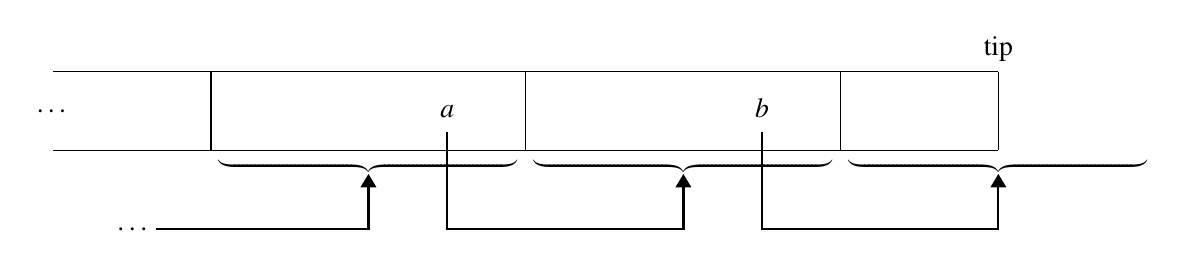
\begin{tikzpicture}
%                             /--------\
%                             |        |
%                             *        v  tip
% 1 -----+------------+------------+-----+
%        |       *    |            |     * current stake
% 0 -----+------------+------------+-----|
%   -10  -8           -4           0     2
%                |          ^
%                \----------/
\draw (-10, 0.5) node{\ldots};
\draw (-10,  0) --  (2, 0);
\draw (-10,  1) --  (2, 1);
\draw  (-8,  0) -- (-8, 1);
\draw  (-4,  0) -- (-4, 1);
\draw   (0,  0) --  (0, 1);
\draw   (2,  0) --  (2, 1) node[above]{tip};
\draw  (-6, -0.2) node {$\underbrace{\hspace{3.8cm}}$};
\draw  (-2, -0.2) node {$\underbrace{\hspace{3.8cm}}$};
\draw  ( 2, -0.2) node {$\underbrace{\hspace{3.8cm}}$};
\draw [thick, arrows={-Triangle}] (-9, -1) node[fill=white] {$\ldots$}-- (-6, -1) -- (-6, -0.3);
\draw [thick, arrows={-Triangle}] (-5, 0.5) node[fill=white] {$\mathstrut a$} -- (-5, -1) -- (-2, -1) -- (-2, -0.3);
\draw [thick, arrows={-Triangle}] (-1, 0.5) node[fill=white] {$\mathstrut b$} -- (-1, -1) -- (2, -1) -- (2, -0.3);
\end{tikzpicture}
\end{center}
%
This makes it possible to \emph{forecast} what the stake distribution (i.e.,
the ledger view) will be at various points. For example, if the chain looks like
%
\begin{center}
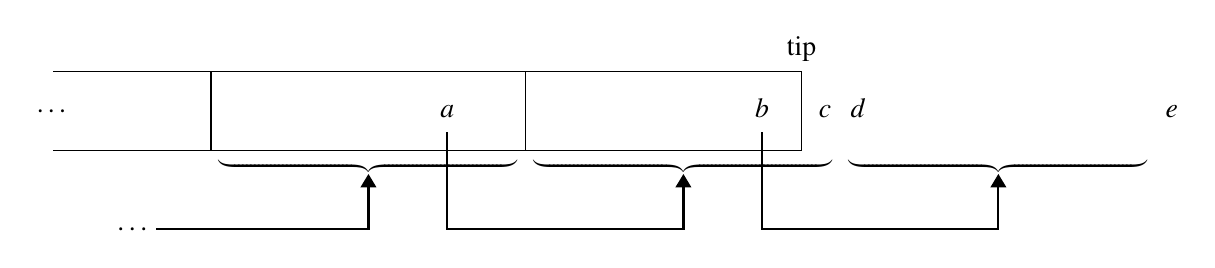
\begin{tikzpicture}
\draw (-10,    0.5) node{\ldots};
\draw (-10,    0) -- (-0.5, 0);
\draw (-10,    1) -- (-0.5, 1);
\draw  (-8,    0) -- (-8,   1);
\draw  (-4,    0) -- (-4,   1);
\draw  (-0.5,  0) -- (-0.5, 1) node[above]{tip};
\draw  (-6,   -0.2) node {$\underbrace{\hspace{3.8cm}}$};
\draw  (-2,   -0.2) node {$\underbrace{\hspace{3.8cm}}$};
\draw  ( 2,   -0.2) node {$\underbrace{\hspace{3.8cm}}$};
\draw [thick, arrows={-Triangle}] (-9, -1) node[fill=white] {$\ldots$}-- (-6, -1) -- (-6, -0.3);
\draw [thick, arrows={-Triangle}] (-5, 0.5) node[fill=white] {$\mathstrut a$} -- (-5, -1) -- (-2, -1) -- (-2, -0.3);
\draw [thick, arrows={-Triangle}] (-1, 0.5) node[fill=white] {$\mathstrut b$} -- (-1, -1) -- (2, -1) -- (2, -0.3);
\draw (0, 0.5) node[left] {$\mathstrut c$};
\draw (0, 0.5) node[right] {$\mathstrut d$};
\draw (4, 0.5) node[right] {$\mathstrut e$};
\end{tikzpicture}
\end{center}
%
then we can ``forecast'' that the stake distribution at point $c$ will be the one
established at point $a$, whereas the stake distribution at point $d$ will be the
one established at point $b$. The stake distribution at point $e$ is however not
yet known; we say that $e$ is ``out of the forecast range''.

\subsection{Code}

Since we're always forecasting what the ledger would look like \emph{if it would
be advanced to a particular slot}, the result of forecasting is always something
ticked:\footnote{An \emph{unticked} ledger view would arise from deriving the
ledger view from the \emph{current} ledger state, not taking (nor needing to
take) into account any changes that have been scheduled for later slots. The
unticked ledger view is however rarely useful; when we validate a header, any
changes that have been scheduled in the most recent ledger state for slots
before or at the slot number of the header must be applied before we validate
the header; we therefore almost exclusively work with ticked ledger views.}
%
\begin{lstlisting}
data Forecast a = Forecast {
      forecastAt  :: WithOrigin SlotNo
    , forecastFor :: SlotNo -> Except OutsideForecastRange (Ticked a)
    }
\end{lstlisting}
%
Here \lstinline!forecastAt! is the tip of the ledger in which the forecast was
constructed and \lstinline!forecastFor! is constructing the forecast for a
particular slot, possibly returning an error message of that slot is out of
range. This terminology---a forecast constructed \emph{at} a slot
and computed \emph{for} a slot---is used throughout both this technical report
as well as the consensus layer code base.

\subsection{Ledger view}
\label{forecast:ledgerview}

For the ledger view specifically, the \lstinline!LedgerSupportsProtocol!
class (\cref{ledger:api:LedgerSupportsProtocol}) requires a function
%
\begin{lstlisting}
ledgerViewForecastAt ::
     LedgerConfig blk
  -> LedgerState blk
  -> Forecast (LedgerView (BlockProtocol blk))
\end{lstlisting}
%
This function must satisfy two important properties:
%
\begin{description}
\item[Sufficient range]

When we validate headers from an upstream node, the most recent usable ledger
state we have is the ledger state at the intersection of our chain and the chain
of the upstream node. That intersection will be at most $k$ blocks back, because
that is our maximum rollback and we disconnect from nodes that fork from our
chain more than $k$ blocks ago (\cref{consensus:overview:k}). Furthermore, it is
only useful to track an upstream peer if we might want to adopt their blocks,
and we only switch to their chain if it is longer than ours
(\cref{consensus:overview:chainsel}). This means that in the worst case
scenario, with the intersection $k$ blocks back, we need to be able to evaluate
$k + 1$ headers in order to adopt the alternative chain. However, the range of a
forecast is based on \emph{slots}, not blocks; since not every slot may contain
a block (\cref{time:slots-vs-blocks}), the range needs to be sufficient to
\emph{guarantee} to contain at least $k + 1$ blocks\footnote{Due to a
misalignment between the consensus requirements and the Sophie specification,
this is not the case for Sophie, where the effective maximum rollback is in
fact $k - 1$; see \cref{sophie:forecasting}).}; we will come back to this in
\cref{future:block-vs-slot}.

The network layer may have additional reasons for wanting a long forecast
range; see \cref{nonfunctional:network:headerbody}.

\item[Relation to ticking]
Forecasting is not the only way that we can get a ledger view for a particular
slot; alternatively, we can also \emph{tick} the ledger state, and then ask
for the ledger view at that ticked ledger state. These two ways should give us
the same answer:
%
\begin{equation}
\begin{array}{lllll}
\mathrm{whenever} &
\mathtt{forecastFor} \; (\mathtt{ledgerViewForecastAt}_\mathit{cfg} \; l) \; s & = & \mathtt{Right} & l' \\
\mathrm{then} & \mathtt{protocolLedgerView}_\mathit{cfg} \; (\mathtt{applyChainTick}_\mathit{cfg} \; s \; l) & = && l'
\end{array}
\end{equation}
%
In other words, whenever the ledger view for a particular slot is within the
forecast range, then ticking the ledger state to that slot and asking for the
ledger view at the tip should give the same answer. Unlike forecasting, however,
ticking has no maximum range. The reason is the following fundamental difference between these two concepts:
%
\begin{quote}
\textbf{(Forecast vs. ticking)} When we \emph{forecast} a ledger view, we are
predicting what that ledger view will be, \emph{no matter which blocks will  be
applied to the chain} between the current tip and the slot of the forecast. By
contrast, when we \emph{tick} a ledger, we are applying any time-related
changes to the ledger state in order to apply the \emph{next} block; in other
words, when we tick to a particular slot, \emph{there \emph{are} no blocks in
between the current tip and the slot we're ticking to}. Since there are no
intervening blocks, there is no uncertainty, and hence no limited range.
\end{quote}
\end{description}

\section{Queries}
\label{ledger:queries}

\section{Abandoned approach: historical states}

\input{chapters/consensus/serialisation.tex}

\part{Storage Layer}

\chapter{Overview}

\section{Components}

\subsection{Consensus protocols}
\label{overview:consensus}

The consensus protocol has two primary responsibilities:
\label{consensus-responsibilities}

\begin{description}
\item[Chain selection] Competing chains arise when two or more nodes extend the
chain with different blocks. This can happen when nodes are not aware of each
other's blocks due to temporarily network delays or partitioning, but depending
on the particular choice of consensus algorithm it can also happen in the normal
course of events. When it happens, it is the responsibility of the consensus
protocol to choose between these competing chains.

\item[Leadership check] In proof-of-work blockchains any node can produce a
block at any time, provided that they have sufficient hashing power. By
contrast, in proof-of-stake time is divided into \emph{slots}, and each slot has
a number of designated \emph{slot leaders} who can produce blocks in that slot.
It is the responsibility of the consensus protocol to decide on this mapping
from slots to slot leaders.
\end{description}

The consensus protocol will also need to maintain its own state; we will discuss
state management in more detail in \cref{storage:inmemory}.

\subsection{Ledger}
\label{overview:ledger}

The role of the ledger is to define what is stored \emph{on} the blockchain.
From the perspective of the consensus layer, the ledger has three primary
responsibilities:

\begin{description}
\item[Applying blocks] The most obvious and most important responsibility of
the ledger is to define how the ledger state changes in response to new blocks,
validating blocks at it goes and rejecting invalid blocks.\

\item[Applying transactions] Similar to applying blocks, the ledger layer also
must provide an interface for applying a single transaction to the ledger state.
This is important, because the consensus layer does not just deal with
previously constructed blocks, but also constructs \emph{new} blocks.

\item[Ticking time] Some parts of the ledger state change due to the passage of
time only. For example, blocks might \emph{schedule} some changes to be applied
later, and then when the relevant slot arrives those changes should be applied,
independent from any blocks.

\item[Forecasting] Some consensus protocols require limited information from the
ledger. In Optimum, for example, a node's probability of being a slot leader is
proportional to its stake, but the stake distribution is something that the
ledger keeps track of. We refer to this as a \emph{view} on the ledger, and we
require not just that the ledger can give us a view on the \emph{current} ledger
state, but also \emph{predict} what that view will be for slots in the near
future. We will discuss the motivation for this requirement in
\cref{nonfunctional:network:headerbody}.
\end{description}

The primary reason for separating out ``ticking'' from applying blocks is that
the consensus layer is responsible to the leadership check
(\cref{consensus-responsibilities}), and when we need to decide if we should be
producing a block in a particular slot, we need to know the ledger state at that
slot (even though we don't have a block for that slot \emph{yet}). It is also
required in the mempool; see \cref{mempool}.

\section{Design Goals}

\subsection{Multiple consensus protocols}
\label{multiple-consensus-protocols}

From the beginning it was clear that we would need support for multiple
consensus algorithms: the Cole era uses a consensus algorithm called
(Permissive) BFT (\cref{bft}) and the Sophie era uses a consensus algorithm
called Optimum (\cref{optimum}). Moreover, the Bcc blockchain is a \emph{hybrid}
chain where the prefix of the chain runs Cole (and thus uses BFT), and then
continues with Sophie (and thus uses Optimum); we will come back to the topic of
composing protocols when we discuss the hard fork combinator (\cref{hfc}). It is
therefore important that the consensus layer abstracts over a choice of
consensus protocol.

\subsection{Support for multiple ledgers}
\label{multiple-ledgers}

For much the same reason that we must support multiple consensus protocols, we
also have to support multiple ledgers. Indeed, we expect more changes in ledger
than in consensus protocol; currently the Bcc blockchain starts with a
Cole ledger and then transitions to a Sophie ledger, but further changes to
the ledger have already been planned (some intermediate ledgers currently
code-named Evie and Jen, as well as larger updates to Charles, Brandon and
Sjobs). All of the ledgers (Sophie up to including Sjobs)
use the Optimum consensus algorithm (potentially extended with the genesis chain
selection rule, see \cref{genesis}).

\subsection{Decouple consensus protocol from ledger}
\label{decouple-consensus-ledger}

As we saw above (\cref{multiple-ledgers}), we have multiple ledgers that all
use the same consensus protocol. We therefore should be able to define the
consensus protocol \emph{independent} from a particular choice of ledger,
merely defining what the consensus protocol expects from the ledger
(we will see what this interface looks like in \cref{ledger}).

\subsection{Testability}
\label{testability}

The consensus layer is a critical component of the Bcc Node, the software
that runs the Bcc blockchain. Since the blockchain is used to run the bcc
cryptocurrency, it is of the utmost importance that this node is reliable;
network downtime or, worse, corruption of the blockchain, cannot be tolerated.
As such the consensus layer is subject to much stricter correctness criteria
than most software, and must be tested thoroughly. To make this possible, we
have to design for testability.

\begin{itemize}
\item We must be able to simulate various kinds of failures (disk
failures, network failures, etc.) and verify that the system can recover.
\item We must be able to run \emph{lots} of tests which means that tests need to
be cheap. This in turn will require for example the possibility to swap the
cryptographic algorithms for much faster ``mock'' crypto algorithms.
\item We must be able to test how the system behaves under certain
expected-but-rare circumstances. For example, under the Optimum consensus
protocol it can happen that a particular slot has multiple leaders. We should be
able to test what happens when this happens repeatedly, but the leader selection
is a probabilistic process; it would be difficult to set up test scenarios to
test for this specifically, and even more difficult to set things up so that
those scenarios are \emph{shrinkable} (leading to minimal test cases). We must
therefore be able to ``override'' the behaviour of the consensus protocol (or
indeed the ledger) at specific points.
\item We must be able to test components individually (rather than just the
system as a whole), so that if a test fails, it is much easier to see where
something went wrong.
\end{itemize}

\subsection{Adaptability and Maintainability}
\label{adaptability}

The Bcc Node began its life as an ambitious replacement of the initial
implementation of the Bcc blockchain, which had been developed by Serokell.
At the time, the Sophie ledger was no more than a on-paper design, and
the Optimum consensus protocol existed only as a research paper. Moreover, since
the redesign would be unable to reuse any parts of the initial implementation,
even the Cole ledger did not yet exist when the consensus layer was started.
It was therefore important from the get-go that the consensus layer was not
written for a specific ledger, but rather abstract over a choice of ledger
and define precisely what the responsibilities of that ledger were.

This abstraction over both the consensus algorithm and the ledger is important
for other reasons, too. As we've mentioned, although initially developed to
support the Cole ledger and the (Permissive) BFT consensus algorithm, the goal
was to move to Sophie/Optimum as quickly as possible. Moreover, additional
ledgers had already been planned (Charles, Brandon and Sjobs), and research on
consensus protocols was (and still is) ongoing. It was therefore important that
the consensus layer could easily be adapted.

Admittedly, adaptability does not \emph{necessarily} require abstraction. We
could have built the consensus layer against the Cole ledger initially
(although we might have had to wait for it to be partially completed at least),
and then generalise as we went. There are however a number of downsides to this
approach.

\begin{itemize}
\item When working with a concrete interface, it is difficult to avoid certain
assumptions creeping in that may hold for this ledger but will not hold for
other ledgers necessarily. When such assumptions go unnoticed, it can be costly
to adjust later. (For one example of such an assumption that nonetheless
\emph{did} go unnoticed, despite best efforts, and took a lot of work to
resolve, see \cref{time} on removing the assumption that we can always
convert between wallclock time and slot number.)

\item TBCO is involved in the development of blockchains other than the public
Bcc instance, and from the start of the project, the hope was that the
consensus layer can be used in those projects as well. Indeed, it is currently
being integrated into various other TBCO projects.

\item Perhaps most importantly, if the consensus layer only supports a single,
concrete ledger, it would be impossible to \emph{test} the consensus layer with
any ledgers other than that concrete ledger. But this means that all consensus
tests need to deal with all the complexities of the real ledger. By contrast,
by staying abstract, we can run a lot of consensus tests with mock ledgers that
are easier to set up, easier to reason about, more easily instrumented and more
amenable to artificially creating rare circumstances (see \cref{testability}).
\end{itemize}

Of course, abstraction is also just good engineering practice. Programming
against an abstract interface means we are clear about our assumptions,
decreases dependence between components, and makes it easier to understand and
work with individual components without having to necessarily understand the
entire system as a whole.

\subsection{Composability}
\label{composability}

The consensus layer is a complex piece of software;  at the time we are writing
this technical report, it consists of roughly 100,000 lines of code. It is
therefore important that we split it into into small components that can be
understood and modified independently from the rest of the system. Abstraction,
discussed in \cref{adaptability}, is one technique to do that, but by no means
the only. One other technique that we make heavy use of is composability. We
will list two examples here:

\begin{itemize}
\item As discussed in \cref{multiple-consensus-protocols} and
\cref{multiple-ledgers}, the Bcc blockchain has a prefix that runs the BFT
consensus protocol and the Cole ledger, and then continues with the Optimum
consensus protocol and the Sophie ledger. We do not however define a consensus
protocol that is the combination of Cole and Optimum, nor a ledger that is the
combination of Cole and Sophie. Instead, the \emph{hard fork combinator}
(\cref{hfc}) makes it possible to \emph{compose} consensus protocols and
ledgers: construct the hybrid consensus protocol from an implementation of BFT
and an implementation of Optimum, and similarly for the ledger.

\item We mentioned in \cref{testability} that it is important that we can
test the behaviour of the consensus layer under rare-but-possible circumstances,
and that it is therefore important that we can override the behaviour of the
consensus algorithm in tests. We do not accomplish this however by adding
special hooks to the Optimum consensus algorithm (or any other); instead we define
another combinator that takes the implementation of a consensus algorithm and
\emph{adds} additional hooks for the sake of the testing infrastructure. This
means that the implementation of Optimum does not have to be aware of testing
constraints, and the combinator that adds these testing hooks does not need to
be aware of the details of how Optimum is implemented.
\end{itemize}

\subsection{Predictable Performance}

Make sure node operators do not set up nodes for "normal circumstances" only
for the network to go down when something infrequent (but expected) occurs.
(This is not about malicious behaviour, that's the next section).

\duncan

\subsection{Protection against DoS attacks}

Brief introduction to asymptotic attacker/defender costs. (This is just an
overview, we come back to these topics in more detail later.)

\duncan

\section{History}
\label{overview:history} % OBFT references refer to this section as well

\duncan

\begin{itemize}
\item Briefly describe the old system (\lstinline!bcc-sl!) the decision
to rewrite it
\item Briefly discuss the OBFT hard fork.
\end{itemize}

\input{chapters/storage/immutabledb.tex}
\input{chapters/storage/volatiledb.tex}
\input{chapters/storage/ledgerdb.tex}
\input{chapters/storage/chainselection.tex}
\input{chapters/storage/chaindb.tex}
\input{chapters/storage/mempool.tex}

\part{Mini protocols}

\input{chapters/miniprotocols/chainsyncclient}
\input{chapters/miniprotocols/servers}

\part{Hard Fork Combinator}

\chapter{Overview}

\section{Components}

\subsection{Consensus protocols}
\label{overview:consensus}

The consensus protocol has two primary responsibilities:
\label{consensus-responsibilities}

\begin{description}
\item[Chain selection] Competing chains arise when two or more nodes extend the
chain with different blocks. This can happen when nodes are not aware of each
other's blocks due to temporarily network delays or partitioning, but depending
on the particular choice of consensus algorithm it can also happen in the normal
course of events. When it happens, it is the responsibility of the consensus
protocol to choose between these competing chains.

\item[Leadership check] In proof-of-work blockchains any node can produce a
block at any time, provided that they have sufficient hashing power. By
contrast, in proof-of-stake time is divided into \emph{slots}, and each slot has
a number of designated \emph{slot leaders} who can produce blocks in that slot.
It is the responsibility of the consensus protocol to decide on this mapping
from slots to slot leaders.
\end{description}

The consensus protocol will also need to maintain its own state; we will discuss
state management in more detail in \cref{storage:inmemory}.

\subsection{Ledger}
\label{overview:ledger}

The role of the ledger is to define what is stored \emph{on} the blockchain.
From the perspective of the consensus layer, the ledger has three primary
responsibilities:

\begin{description}
\item[Applying blocks] The most obvious and most important responsibility of
the ledger is to define how the ledger state changes in response to new blocks,
validating blocks at it goes and rejecting invalid blocks.\

\item[Applying transactions] Similar to applying blocks, the ledger layer also
must provide an interface for applying a single transaction to the ledger state.
This is important, because the consensus layer does not just deal with
previously constructed blocks, but also constructs \emph{new} blocks.

\item[Ticking time] Some parts of the ledger state change due to the passage of
time only. For example, blocks might \emph{schedule} some changes to be applied
later, and then when the relevant slot arrives those changes should be applied,
independent from any blocks.

\item[Forecasting] Some consensus protocols require limited information from the
ledger. In Optimum, for example, a node's probability of being a slot leader is
proportional to its stake, but the stake distribution is something that the
ledger keeps track of. We refer to this as a \emph{view} on the ledger, and we
require not just that the ledger can give us a view on the \emph{current} ledger
state, but also \emph{predict} what that view will be for slots in the near
future. We will discuss the motivation for this requirement in
\cref{nonfunctional:network:headerbody}.
\end{description}

The primary reason for separating out ``ticking'' from applying blocks is that
the consensus layer is responsible to the leadership check
(\cref{consensus-responsibilities}), and when we need to decide if we should be
producing a block in a particular slot, we need to know the ledger state at that
slot (even though we don't have a block for that slot \emph{yet}). It is also
required in the mempool; see \cref{mempool}.

\section{Design Goals}

\subsection{Multiple consensus protocols}
\label{multiple-consensus-protocols}

From the beginning it was clear that we would need support for multiple
consensus algorithms: the Cole era uses a consensus algorithm called
(Permissive) BFT (\cref{bft}) and the Sophie era uses a consensus algorithm
called Optimum (\cref{optimum}). Moreover, the Bcc blockchain is a \emph{hybrid}
chain where the prefix of the chain runs Cole (and thus uses BFT), and then
continues with Sophie (and thus uses Optimum); we will come back to the topic of
composing protocols when we discuss the hard fork combinator (\cref{hfc}). It is
therefore important that the consensus layer abstracts over a choice of
consensus protocol.

\subsection{Support for multiple ledgers}
\label{multiple-ledgers}

For much the same reason that we must support multiple consensus protocols, we
also have to support multiple ledgers. Indeed, we expect more changes in ledger
than in consensus protocol; currently the Bcc blockchain starts with a
Cole ledger and then transitions to a Sophie ledger, but further changes to
the ledger have already been planned (some intermediate ledgers currently
code-named Evie and Jen, as well as larger updates to Charles, Brandon and
Sjobs). All of the ledgers (Sophie up to including Sjobs)
use the Optimum consensus algorithm (potentially extended with the genesis chain
selection rule, see \cref{genesis}).

\subsection{Decouple consensus protocol from ledger}
\label{decouple-consensus-ledger}

As we saw above (\cref{multiple-ledgers}), we have multiple ledgers that all
use the same consensus protocol. We therefore should be able to define the
consensus protocol \emph{independent} from a particular choice of ledger,
merely defining what the consensus protocol expects from the ledger
(we will see what this interface looks like in \cref{ledger}).

\subsection{Testability}
\label{testability}

The consensus layer is a critical component of the Bcc Node, the software
that runs the Bcc blockchain. Since the blockchain is used to run the bcc
cryptocurrency, it is of the utmost importance that this node is reliable;
network downtime or, worse, corruption of the blockchain, cannot be tolerated.
As such the consensus layer is subject to much stricter correctness criteria
than most software, and must be tested thoroughly. To make this possible, we
have to design for testability.

\begin{itemize}
\item We must be able to simulate various kinds of failures (disk
failures, network failures, etc.) and verify that the system can recover.
\item We must be able to run \emph{lots} of tests which means that tests need to
be cheap. This in turn will require for example the possibility to swap the
cryptographic algorithms for much faster ``mock'' crypto algorithms.
\item We must be able to test how the system behaves under certain
expected-but-rare circumstances. For example, under the Optimum consensus
protocol it can happen that a particular slot has multiple leaders. We should be
able to test what happens when this happens repeatedly, but the leader selection
is a probabilistic process; it would be difficult to set up test scenarios to
test for this specifically, and even more difficult to set things up so that
those scenarios are \emph{shrinkable} (leading to minimal test cases). We must
therefore be able to ``override'' the behaviour of the consensus protocol (or
indeed the ledger) at specific points.
\item We must be able to test components individually (rather than just the
system as a whole), so that if a test fails, it is much easier to see where
something went wrong.
\end{itemize}

\subsection{Adaptability and Maintainability}
\label{adaptability}

The Bcc Node began its life as an ambitious replacement of the initial
implementation of the Bcc blockchain, which had been developed by Serokell.
At the time, the Sophie ledger was no more than a on-paper design, and
the Optimum consensus protocol existed only as a research paper. Moreover, since
the redesign would be unable to reuse any parts of the initial implementation,
even the Cole ledger did not yet exist when the consensus layer was started.
It was therefore important from the get-go that the consensus layer was not
written for a specific ledger, but rather abstract over a choice of ledger
and define precisely what the responsibilities of that ledger were.

This abstraction over both the consensus algorithm and the ledger is important
for other reasons, too. As we've mentioned, although initially developed to
support the Cole ledger and the (Permissive) BFT consensus algorithm, the goal
was to move to Sophie/Optimum as quickly as possible. Moreover, additional
ledgers had already been planned (Charles, Brandon and Sjobs), and research on
consensus protocols was (and still is) ongoing. It was therefore important that
the consensus layer could easily be adapted.

Admittedly, adaptability does not \emph{necessarily} require abstraction. We
could have built the consensus layer against the Cole ledger initially
(although we might have had to wait for it to be partially completed at least),
and then generalise as we went. There are however a number of downsides to this
approach.

\begin{itemize}
\item When working with a concrete interface, it is difficult to avoid certain
assumptions creeping in that may hold for this ledger but will not hold for
other ledgers necessarily. When such assumptions go unnoticed, it can be costly
to adjust later. (For one example of such an assumption that nonetheless
\emph{did} go unnoticed, despite best efforts, and took a lot of work to
resolve, see \cref{time} on removing the assumption that we can always
convert between wallclock time and slot number.)

\item TBCO is involved in the development of blockchains other than the public
Bcc instance, and from the start of the project, the hope was that the
consensus layer can be used in those projects as well. Indeed, it is currently
being integrated into various other TBCO projects.

\item Perhaps most importantly, if the consensus layer only supports a single,
concrete ledger, it would be impossible to \emph{test} the consensus layer with
any ledgers other than that concrete ledger. But this means that all consensus
tests need to deal with all the complexities of the real ledger. By contrast,
by staying abstract, we can run a lot of consensus tests with mock ledgers that
are easier to set up, easier to reason about, more easily instrumented and more
amenable to artificially creating rare circumstances (see \cref{testability}).
\end{itemize}

Of course, abstraction is also just good engineering practice. Programming
against an abstract interface means we are clear about our assumptions,
decreases dependence between components, and makes it easier to understand and
work with individual components without having to necessarily understand the
entire system as a whole.

\subsection{Composability}
\label{composability}

The consensus layer is a complex piece of software;  at the time we are writing
this technical report, it consists of roughly 100,000 lines of code. It is
therefore important that we split it into into small components that can be
understood and modified independently from the rest of the system. Abstraction,
discussed in \cref{adaptability}, is one technique to do that, but by no means
the only. One other technique that we make heavy use of is composability. We
will list two examples here:

\begin{itemize}
\item As discussed in \cref{multiple-consensus-protocols} and
\cref{multiple-ledgers}, the Bcc blockchain has a prefix that runs the BFT
consensus protocol and the Cole ledger, and then continues with the Optimum
consensus protocol and the Sophie ledger. We do not however define a consensus
protocol that is the combination of Cole and Optimum, nor a ledger that is the
combination of Cole and Sophie. Instead, the \emph{hard fork combinator}
(\cref{hfc}) makes it possible to \emph{compose} consensus protocols and
ledgers: construct the hybrid consensus protocol from an implementation of BFT
and an implementation of Optimum, and similarly for the ledger.

\item We mentioned in \cref{testability} that it is important that we can
test the behaviour of the consensus layer under rare-but-possible circumstances,
and that it is therefore important that we can override the behaviour of the
consensus algorithm in tests. We do not accomplish this however by adding
special hooks to the Optimum consensus algorithm (or any other); instead we define
another combinator that takes the implementation of a consensus algorithm and
\emph{adds} additional hooks for the sake of the testing infrastructure. This
means that the implementation of Optimum does not have to be aware of testing
constraints, and the combinator that adds these testing hooks does not need to
be aware of the details of how Optimum is implemented.
\end{itemize}

\subsection{Predictable Performance}

Make sure node operators do not set up nodes for "normal circumstances" only
for the network to go down when something infrequent (but expected) occurs.
(This is not about malicious behaviour, that's the next section).

\duncan

\subsection{Protection against DoS attacks}

Brief introduction to asymptotic attacker/defender costs. (This is just an
overview, we come back to these topics in more detail later.)

\duncan

\section{History}
\label{overview:history} % OBFT references refer to this section as well

\duncan

\begin{itemize}
\item Briefly describe the old system (\lstinline!bcc-sl!) the decision
to rewrite it
\item Briefly discuss the OBFT hard fork.
\end{itemize}

\input{chapters/hfc/time.tex}
\input{chapters/hfc/misc.tex}

\part{Testing}

\input{chapters/testing/consensus.tex}
\input{chapters/testing/storage.tex}

\part{Future Work}

\input{chapters/future/genesis.tex}
\input{chapters/future/lowdensity.tex}
\input{chapters/future/ebbs.tex}
\input{chapters/future/misc.tex}

\part{Conclusions}

\input{chapters/conclusions/technical.tex}
\input{chapters/conclusions/conclusions}

\part{Appendices}
\appendix

\chapter{Cole}

Some details specific to the Cole ledger.
EBBs already discussed at length in \cref{ebbs}.

The Cole specification can be found at \url{https://github.com/The-Blockchain-Company/bcc-ledger-specs}.

\section{Update proposals}
\label{cole:hardfork}

\subsection{Moment of hard fork}
\label{cole:hardfork:moment}

The Cole ledger state provides the current protocol version in
%
\begin{lstlisting}
adoptedProtocolVersion :: ProtocolVersion
\end{lstlisting}
%
in the \lstinline!State! type from
\lstinline!Bcc.Chain.Update.Validation.Interface!.
This protocol version is a three-tuple \emph{major}, \emph{minor}, \emph{alt}.
The Cole specification does not provide any semantic interpretation of these
components. By convention (outside of the purview of the Cole specification),
the hard fork is initiated the moment that the \emph{major} component of
\lstinline!adoptedProtocolVersion! reaches a predefined, hardcoded, value.

\subsection{The update mechanism for the \lstinline!ProtocolVersion!}

Updates to the \lstinline!ProtocolVersion! in Cole are part of the general
infrastructure for changing protocol parameters (parameters such as the maximum
block size), except that in the case of a hard fork, we care only about changing
the \lstinline!ProtocolVersion!, and not any of the parameters themselves.

The general mechanism for updating protocol parameters in Cole is as follows:

\begin{enumerate}

\item
A protocol update \emph{proposal} transaction is created. It proposes new values
for some protocol parameters and a greater \emph{protocol version} number as an
identifier. There cannot be two proposals with the same version number.

\item
Genesis key delegates can add \emph{vote} transactions that refer to such a
proposal (by its hash). They don't have to wait; a node could add a proposal and
a vote for it to its mempool simultaneously. There are only positive votes, and
a proposal has a time-to-live (see \lstinline!ppUpdateProposalTTL!) during which
to gather sufficient votes. While gathering votes, a proposal is called
\emph{active}.

Note that neither Cole nor Sophie support full centralisation (everybody can
vote); this is what the Sjobs ledger is intended to accomplish.

\item
Once the number of voters satisfies a threshold (currently determined by the
\lstinline!srMinThd! field of the \lstinline!ppSoftforkRule! protocol
parameter), the proposal becomes \emph{confirmed}.

\item
Once the threshold-satisfying vote becomes stable (i.e. its containing block is at
least $2k$ slots deep), a block whose header's protocol version number
(\lstinline!CC.Block.headerProtocolVersion!) is that of the proposal is
interpreted as an \emph{endorsement} of the stably-confirmed proposal by the
block's issuer (specifically by the Verification Key of its delegation
certificate). Endorsements---i.e. \emph{any block}, since they all contain that
header field---also trigger the system to discard proposals that were not
confirmed within their TTL.

Notably, endorsements for proposals that are not yet stably-confirmed (or do not
even exist) are not invalid but rather silently ignored. In other words, no
validation applies to the `headerProtocolVersion` field.

\item
Once the number of endorsers satisfies a threshold (same as for voting), the
confirmed proposal becomes a \emph{candidate} proposal.

\item
\emph{At the beginning of an epoch}, the candidate proposal with the greatest
protocol version number among those candidates whose threshold-satisfying
endorsement is stable (i.e. the block is at least $2k$ deep) is \emph{adopted}:
the new protocol parameter values have now been changed.

If there was no stable candidate proposal, then nothing happens. Everything is
retained; in particular, a candidate proposal whose threshold-satisfying
endorsement was not yet stable will be adopted at the subsequent epoch unless it
is surpassed in the meantime.

When a candidate is adopted, all record of other
proposals/votes/endorsements---regardless of their state---is discarded. The
explanation for this is that such proposals would now be interpreted as an
update to the newly adopted parameter values, whereas they were validated as an
update to the previously adopted parameter values.

\end{enumerate}

The diagram shown in \cref{cole:update-process} summarises the progress of a
proposal that's eventually adopted. For other proposals, the path short circuits
to a ``rejected/discarded'' status at some point.

\begin{figure}
\hrule
\begin{center}
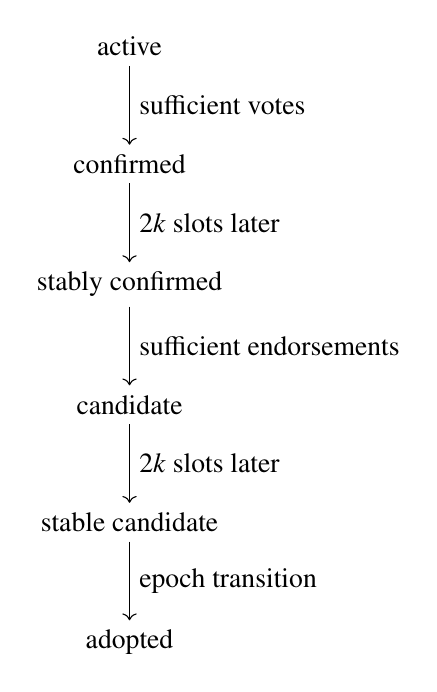
\begin{tikzpicture}
\node (act)                {active}           ;
\node (con) [below=of act] {confirmed}        ;
\node (sta) [below=of con] {stably confirmed} ;
\node (can) [below=of sta] {candidate}        ;
\node (sca) [below=of can] {stable candidate} ;
\node (ado) [below=of sca] {adopted}          ;
\draw[->] (act.south) -- (con.north) node[pos=0.5, right] {sufficient votes};
\draw[->] (con.south) -- (sta.north) node[pos=0.5, right] {$2k$ slots later};
\draw[->] (sta.south) -- (can.north) node[pos=0.5, right] {sufficient endorsements};
\draw[->] (can.south) -- (sca.north) node[pos=0.5, right] {$2k$ slots later};
\draw[->] (sca.south) -- (ado.north) node[pos=0.5, right] {epoch transition};
\end{tikzpicture}
\end{center}
\hrule
\caption{\label{cole:update-process}Cole update proposal process}
\end{figure}

\subsection{Initiating the hard fork}
\label{cole:hardfork:initiating}

Proposals to initiate the hard fork can be submitted and voted on before all
core nodes are ready. After all, once a proposal is stably confirmed, it will
effectively remain so indefinitely until nodes endorse it (or it gets superseded
by another proposal). This means that nodes can vote to initiate the hard fork,
\emph{then} wait for everybody to update their software, and once updated, the
proposal is endorsed and eventually the hard fork is initiated.

Endorsement is somewhat implicit. The node operator does not submit an explicit
``endorsement transaction'', but instead restarts the
node\footnote{\label{cole:unnecessary-restarts}A node restart is necessary for
\emph{any} change to a protocol parameter, even though most parameters do not
require any change to the software at all.} (probably after a software update
that makes the node ready to support the hard fork) with a new protocol version
(as part of a configuration file or command line parameter), which then gets included
in the blocks that the node produces (this value is the
\lstinline!coleProtocolVersion! field in the static \lstinline!ColeConfig!).

\subsection{Software versions}

The Cole ledger additionally also records the latest version of the software on
the chain, in order to facilitate software discovering new versions and
subsequently updating themselves. This would normally precede all of the above,
but as far as the consensus layer is concerned, this is entirely orthogonal. It
does not in any way interact with either the decision to hard fork nor the
moment of the hard fork. If we did forego it, the discussion above would still
be entirely correct. As of Sophie, software discovery is done off-chain.

The Cole \emph{block header} also records a software version
(\lstinline!headerSoftwareVersion!). This is a legacy concern only, and is
present in but ignored by the current Cole implementation, and entirely absent
from the Cole specification.

\input{chapters/appendix/sophie.tex}

\bibliographystyle{acm}
\bibliography{references}

\end{document}
